% Chapter 1

\chapter{Introduction} % Main chapter title
%\addchaptertocentry{Introduction} 
\label{Introduction} % For referencing the chapter elsewhere, use \ref{Chapter1} 

%----------------------------------------------------------------------------------------

% Define some commands to keep the formatting separated from the content 
\newcommand{\keyword}[1]{\textbf{#1}}
\newcommand{\tabhead}[1]{\textbf{#1}}
\newcommand{\code}[1]{\texttt{#1}}
\newcommand{\file}[1]{\texttt{\bfseries#1}}
\newcommand{\option}[1]{\texttt{\itshape#1}}

%----------------------------------------------------------------------------------------

\section{Vision naturelle}
% Rôle de la vision
Tous  les êtres vivants utilisent la vision à un degré ou à un autre, et pour de nombreuses espèces -y compris la notre- elle est même la modalité perceptive principale. Elle est alors primordiale pour appréhender l'environnement et interagir avec celui-ci, que ce soit dans une optique de survie de l'individu ou dans la construction de relations sociales.\\

% Structure générale d'une rétine (cônes/bâtonnets + fovéa/rétine périphérique)
Chez les vertébrés la vision débute à la surface de la rétine, où les cellules photovoltaïques (cônes et bâtonnets) réalisent la transduction des signaux lumineux qui les atteignent en signaux électriques, transmissibles au réseaux nerveux en aval.\\
Les cônes et les bâtonnets sont différenciables par un certain nombre de caractéristiques, notamment leur sensibilité aux longueurs d'ondes lumineuses et leur distribution au sein de la rétine. Ces différences permettent à notre rétine de rester fonctionnelle dans de nombreuses situations, y compris lorsque la luminance est très faible (le seuil absolu de la rétine humaine correspondant à 70 photons) et lui permet donc de nous fournir des informations pertinentes dans une grande variété de contextes.\\
Le champs visuel peut être divisé en deux parties. La vision centrale (environ \SI{2}{\degree} chez l'humain) est soutenue par la fovea, une région rétinienne comprenant uniquement des cônes. On y observe l'acuité visuelle la plus importante (la région présente les champs récépteurs les plus petits de la rétine).\\
La vision périphérique comprends majoritairement des bâtonnets, présente une faible acuité et une perception des couleurs très faible (voir nulle). Elle est par contre très sensible à des variations de luminance et de fréquence spatiale (donc aux mouvements ;  \cite{Werner2014}).\\
 L'acuité visuelle diminue en fait avec l'excentricité par rapport à la fovéa. Autrement dit, les champs récepteurs visuels grandissent avec cette excentricité.

% Notion de saccades oculaires/Vision d'une cible en périphérie
Lors de l'exploration de son environnement visuel, un agent va pouvoir détecter des stimuli dans sa vision périphérique mais ne va pas y présenter assez d'acuité pour réaliser une description précise.
En conséquences, l'agent va réaliser des saccades oculaires (mouvements brefs (20-60\si{\milli\second}) des globes oculaires) afin de placer l'image de la cible (ou tout du moins sa position prédite dans l'espace) au niveau de la fovéa, permettant ainsi de traiter les informations en provenant avec la plus grande précision possible.\\

% Cellules parvo/magno -> rôle de la voie magno
L'activité rétinienne est transmise le long des voies nerveuses visuelles jusqu'au cortex visuel, où sera réalisé la majorité du traitement des informations -notamment haut niveau- qu'elle code. \\
Entre la rétine et le cortex existe un certain nombre d'étapes, mais tout au long de ces voies la distribution rétinienne de l'information (la rétinotopie) est conservée. 

\begin{figure}[th]
\centering
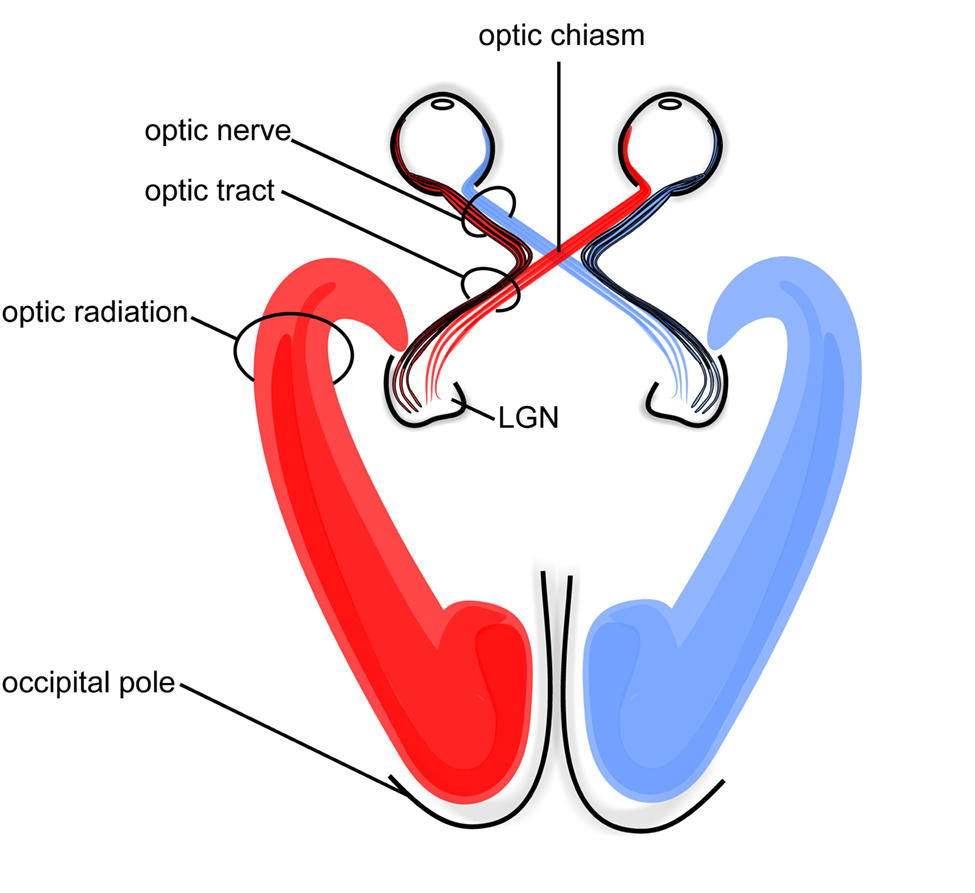
\includegraphics{Figures/visual_system}
\decoRule %puts an aesthetic horizontal line below the image
\caption[Figure]{Schéma des voies visuelles précorticales humaines (adapté de Hofer S. et al., 2010 via Wikimedia Commons [CC BY 3.0])}
\label{fig:visual_system}
\end{figure}

Dans leurs travaux de 1962 et 1977, Hubel et Wiesel émettent l'hypothèse des courants visuels. Cette hypothèse définit trois voies nerveuses naissant dans le \textbf{corps genouillé latéral} (LGN, où sont présents les corps des types cellulaires donnant leurs noms aux voies) et projetant sur le \textbf{cortex visuel primaire} (V1) :  \textbf{magnocellulaire} (M),  \textbf{parvocellulaire} (P) et  \textbf{koniocellulaire} (K). Chacune de ces voies supporte le transport d'informations codant pour des caractéristiques différentes des stimuli visuels.\\
L'activité des cellules M ne distingue pas les couleurs mais est sensible à des différences fines de luminance, de contraste et de fréquence spatiale. Ces caractèristiques semblent lier la voie M notamment au traitement de la luminance et des mouvements (\cite{Werner2014}).

% Voie dorsale, rôle dans la localisation de cible et les saccades oculaires
Cette multiplicité de voies visuelles réalisant des traitements différents des stimuli est conservée au delà de V1, où l'on décrit deux courant sortants : la \textbf{voie ventrale} (transportant et traitant majoritairement pour des informations provenant de la voie P) et la \textbf{voie dorsale} (transportant et traitant majoritairement pour des informations provenant de la voie M).\\
La voie ventrale communique ainsi principalement avec les aires cérébrales du lobe temporal, l'activité de son réseau étant primordiale pour la reconnaissance et l'identification des objets visuels. La voie dorsale quant à elle communique principalement avec les aires du lobe pariétal, l'activité de ce réseau étant primordiale pour le traitement des relations spatiales entre les objets visuels ainsi que pour le guidage attentionnel et physique vers eux (\cite{Werner2014}).\\
Parmi ce réseau dorsal, on trouve l'\textbf{aire intrapariétale latérale} (LIP), qui recoit en partie des informations directement depuis V1 et V2 (contournant donc le traitement d'aires en amont, dont l'aire MT) codant pour des stimuli dans le champs visuel périphérique. Des travaux ont d'ailleurs relié l'activité des neurones du LIP à la plannification des saccades oculaires et à la représentation spatiale des objets visuels.

%----------------------------------------------------------------------------------------

\section{Vision artificielle}
% Motivations\\
La vision représentant notre modalité perceptive principale et les aire dévouées à traiter ses informations occupant une part significative de notre système nerveux central (environ 50\% chez certains primates ; \cite{Zhaoping2014}), l'étudier permet de mieux comprendre le fonctionnement général de notre système nerveux.\\
De nombreux domaines d'étude s'intéressent donc au fonctionnement du système visuel. Parmi eux, les neuromathématiques se basent sur les données expérimentales (anatomique, physiologique et comportementale) pour émettre des modèles mathématiques sur le fonctionnement d'une partie ou de l'ensemble de la modalité visuelle. Idéalement, ces théories doivent pouvoir expliquer son activité dans l'ensemble des contextes observables, mais aussi pouvoir prédire son comportement dans de nouveaux contextes (\cite{Zhaoping2014}).\\
Mais ces modèles ne sont pas une finalité en soi dans la compréhension du système. Ils peuvent permettre d'identifier dans les théories de son fonctionnement des défauts ou des zones obscures à notre compréhension et donc diriger les études expérimentales vers ces points (\cite{Zhaoping2014}).\\
L'identification de ces points et la démonstration de ces théories peut passer par le domaine des neurosciences computationnelles, qui va tenter d'appliquer ces modèles mathématiques dans des modélisations du système nerveux. Au delà de la possible validation ou invalidation des modèles, les neurosciences computationnelles permettent de résoudre des problèmes d'ingénierie (puissance de calcul disponible, vitesse de traitement, adaptabilité à l'environnement, \ldots) en s'inspirant des systèmes biologiques, très optimisés, et donc de créer des systèmes artificiels neuromimétiques plus performants et intégrables dans des systèmes embarqués ou des interfaces cerveau-machine.\\

%Valider l'une des théories neurofonctionnelles de la détection de cible visuelle.
Dans cette étude, nous avons tenté de construire un modèle simple de localisation de cible visuelle dans un champs rétinien : le modèle possède une vision centrale où son acuité est maximale et une vision périphérique dont l'acuité diminue avec l'excentricité.\\
Le modèle doit être capable de détecter dans sa vision périphérique une cible visuelle aux caractéristiques simples (représentée par un stimulus provenant le base de données MNIST), de prédire précisémment sa position et de réaliser une saccade oculaire afin de la placer dans sa fovea, ce qui lui permet alors de l'identifier avec une certitude élevée.\\
Pour cela plusieurs méthodes (comprenant elles-mêmes plusieurs sous-méthodes) s'offrent à nous. Les \textbf{modèles de saillance} où l'on tente de décrire une image en fonction des régions (ou pixels) qui présentent la plus grande probabilité de fournir des informations pertinentes et donc qui devraient attirer les saccades. Ces modèles permettent donc de créer des histogrammes de probabilité de fixations oculaires mais présentent un certaines limites, dont le fait qu'ils ne vont pas cibler d'objets partiellement ou entièrements cachés (\cite{Butko2010}).\\
Les \textbf{modèles de contrôle}, tentent quant à eux de prédire quelles règles le système devra suivre pour répondre au mieux à une tache. A chaque saccade, de nouvelles informations sur l'environnement sont collectées et permettent de changer l'opinion de l'agent sur le monde (\cite{Butko2010}).
